\documentclass[resume]{subfiles}

\begin{document}
\begin{multicols}{2}
\section{Exercices}
\begin{center}
\begin{tabular}{p{6cm}l}
Résoudre l'équation d'onde sans CB & \ref{S2E1}\\
Équation de diffusion avec CI, sans CB & \ref{S3E2}\\
Équation de diffusion avec CI, sans CB & \ref{S3E3}\\
Équation de diffusion avec CI, sans CB, séparation $p$ / $q$ & \ref{S3E4}\\
Diffusion avec CB mixtes & \ref{S4E4}\\
Onde avec CB mixtes & \ref{S4E5}\\
Polynôme quadratique & \ref{S5E1}\\
Fourier & \ref{S6E2}\\
Onde + Fourier & \ref{S6E5}\\
Laplace & \ref{S7E4}\\

\end{tabular}
\end{center}
\subsection{Série 2 - Exercice 1}
\label{S2E1}
\begin{figure}[H]
\centering
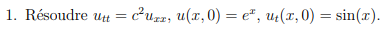
\includegraphics[scale=0.5]{img_8.png}
\end{figure}
On utilise la fonction générale
\begin{multline*}
u(x,t)=\frac{1}{2}(\phi(x+ct)+\phi(x-ct))+\frac{1}{2c}\int_{x-ct}^{x+ct}\sin(s)ds=\\\frac{1}{2}\left(e^{x+ct}+e^{x-ct}\right)+\frac{1}{2c}\left(-\cos(x+ct)+\cos(x-ct)\right)
\end{multline*}
On peut simplifier un peu les expressions
\begin{multline*}
\frac{1}{2}\left(e^{x+ct}+e^{x-ct}\right)+\underbrace{\frac{1}{2c}\left(-\cos(x+ct)+\cos(x-ct)\right)}_{\frac{1}{2}\left(\sin(x)\sin(ct)\right)}=\\e^{x}\underbrace{\frac{1}{2}\left(e^{ct}+e^{-ct}\right)}_{\cosh(ct)}+\frac{1}{2}\sin(x)\sin(ct)
\end{multline*}
\subsection{Série 3 - Exercice 2}
\label{S3E2}
\begin{figure}[H]
\centering
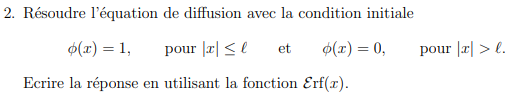
\includegraphics[scale=0.5]{img_9.png}
\end{figure}
On utilise la fonction de base

$$u(x,t)=\frac{1}{2\sqrt{\pi kt}}\int_{-\infty}^{\infty}e^{-\frac{(x-y)^2}{4kt}}\phi(y)dy$$
On applique la fonction $\phi(x)$
$$u(x,t)=\frac{1}{2\sqrt{\pi kt}}\int_{-l}^{l}e^{-\frac{(x-y)^2}{4kt}}dy$$
Puis on effectue un changement de variable $p(y)=\frac{x-y}{\sqrt{4kt}}$
$$dy=-\sqrt{4kt}dp\qquad l\to \frac{x-l}{\sqrt{4kt}}\qquad -l\to\frac{x+l}{\sqrt{4kt}}$$
$$u(x,t)=\frac{-\sqrt{4kt}}{2\sqrt{\pi kt}}\int_{\frac{x+l}{\sqrt{4kt}}}^{\frac{x-l}{\sqrt{4kt}}}e^{-p^2}dp=\frac{-1}{\sqrt{\pi}}\int_{\frac{x+l}{\sqrt{4kt}}}^{\frac{x-l}{\sqrt{4kt}}}e^{-p^2}dp$$
On inverse les bornes (et le signe devant l'intégrale)
$$u(x,t)=\frac{1}{\sqrt{\pi}}\int_{\frac{x-l}{\sqrt{4kt}}}^{\frac{x+l}{\sqrt{4kt}}}e^{-p^2}dp$$
On utilise la fonction erf
$$\text{erf}(x)=\frac{2}{\sqrt{\pi}}\int_{0}^{x}e^{-p^2}dp$$
$$u(x,t)=\frac{1}{\sqrt{\pi}}\left(\frac{\sqrt{\pi}}{2}\text{erf}\left(\frac{x+l}{\sqrt{4kt}}\right)-\frac{\sqrt{\pi}}{2}\text{erf}\left(\frac{x-l}{\sqrt{4kt}}\right)\right)$$

$$\boxed{u(x,t)=\frac{1}{2}\left(\text{erf}\left(\frac{x+l}{\sqrt{4kt}}\right)-\text{erf}\left(\frac{x-l}{\sqrt{4kt}}\right)\right)}$$
(même chose que le corrigé)
\subsection{Série 3 - Exercice 3}
\label{S3E3}
\begin{figure}[H]
\centering
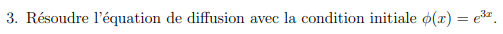
\includegraphics[scale=0.5]{img_10.png}
\end{figure}
On commence par poser l'équation de base
$$u(x,t)=\frac{1}{2\sqrt{\pi kt}}\int_{-\infty}^{\infty}e^{-\frac{(x-y)^2}{4kt}}\phi(y)dy$$
On remplace par l'expression de $\phi(y)$
\begin{multline*}
u(x,t)=\frac{1}{2\sqrt{\pi kt}}\int_{-\infty}^{\infty}e^{-\frac{(x-y)^2}{4kt}}e^{3y}dy=\frac{1}{2\sqrt{\pi kt}}\int_{-\infty}^{\infty}e^{-\frac{(x-y)^2}{4kt}+3y}dy=\\\frac{1}{2\sqrt{\pi kt}}\int_{-\infty}^{\infty}e^{-\frac{(x-y)^2-12kty}{4kt}}dy
\end{multline*}
On doit enlever le terme $12kty$ qui empêche de faire la simplification avec erf. On s'intéresse à la puissance de $e$ et on utilise $(y+2kt-x)^2$ (dans le résumé)
$$-\frac{(x-y)^2-12kty}{4kt}=-\frac{x^2-2xy+y^2-12kty}{4kt}$$
$$(y+2kt-x)^2=y^2+4k^2t^2+x^2+4kty-4ktx-2xy$$
ça ressemble un peu mais on aimerait $-12kty$ au lieu de $4kty$, on inverse $x$ et $y$ et on multiplie le terme central par $3$
$$(x+6kt-y)^2=y^2+36k^2t^2+x^2+12ktx-12kty-2xy$$
C'est parfait, on a plus qu'à adapter l'équation de base pour utiliser ce terme
$$-\frac{(x+6kt-y)^2 - 36k^2t^2-12ktx}{4kt}=-\frac{x^2-2xy+y^2-12kty}{4kt}$$
Maintenant qu'on a le bon terme, il suffit de séparer pour garder les $y$ d'un seul côté
$$-\frac{(x+6kt-y)^2}{4kt} + \frac{36k^2t^2+12ktx}{4kt}=-\frac{(x+6kt-y)^2}{4kt} + 9kt+3x$$
On a plus qu'à remettre tout ça dans l'équation de base et résoudre
$$\frac{1}{2\sqrt{\pi kt}}\int_{-\infty}^{\infty}e^{-\frac{(x+6kt-y)^2}{4kt} + 9kt+3x}dy=\frac{1}{2\sqrt{\pi kt}}\int_{-\infty}^{\infty}e^{-\left(\frac{x+6kt-y}{\sqrt{4kt}}\right)^2}e^{9kt+3x}dy$$
Comme le dernier terme ne dépend pas de $y$, on le sort
$$e^{9kt+3x}\frac{1}{2\sqrt{\pi kt}}\int_{-\infty}^{\infty}e^{-\left(\frac{x+6kt-y}{\sqrt{4kt}}\right)^2}dy$$
On effectue le changement de variable
$$p(y)=\frac{x+6kt-y}{\sqrt{4kt}}\longrightarrow \begin{cases}\infty\to-\infty\\-\infty\to\infty\\dy\to -\sqrt{4kt}dp\end{cases}$$
$$e^{9kt+3x}\frac{-\sqrt{4kt}}{2\sqrt{\pi kt}}\int_{\infty}^{-\infty}e^{-p^2}dy=e^{9kt+3x}\frac{-1}{\sqrt{\pi}}\int_{\infty}^{-\infty}e^{-p^2}dy$$
On inverse les bornes (et le signe au début)
$$u(x,t)=e^{9kt+3x}\frac{1}{\sqrt{\pi}}\underbrace{\int_{-\infty}^{\infty}e^{-p^2}dy}_{\sqrt{\pi}}$$
On a donc finalement
$$\boxed{u(x,t)=e^{9kt+3x}}$$
\subsection{Série 3 - Exercice 4}
\label{S3E4}
\begin{figure}[H]
\centering
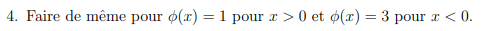
\includegraphics[scale=0.5]{img_11.png}
\end{figure}

On commence par poser l'équation de base

$$u(x,t)=\frac{1}{2\sqrt{\pi kt}}\int_{-\infty}^{\infty}e^{-\frac{(x-y)^2}{4kt}}\phi(y)dy$$
On applique la fonction $\phi(y)$ et on trouve deux intégrales
$$u(x,t)=\frac{1}{2\sqrt{\pi kt}}\left(3\int_{-\infty}^{0}e^{-\frac{(x-y)^2}{4kt}}dy+\int_{0}^{\infty}e^{-\frac{(x-y)^2}{4kt}}dy\right)$$
\begin{mdframed}[linewidth=2pt,linecolor=OrangeRed!50!White]Important ! : on va effectuer deux changements de variables différents pour simplifier les calculs par la suite (voir le résumé)
\end{mdframed}
$$p=\frac{x-y}{\sqrt{4kt}}\qquad q=\frac{y-x}{\sqrt{4kt}}$$
$$u(x,t)=\frac{1}{2\sqrt{\pi kt}}\left(-3\sqrt{4kt}\int_{\infty}^{\frac{x}{\sqrt{4kt}}}e^{-p^2}dp+\sqrt{4kt}\int_{-\frac{x}{\sqrt{4kt}}}^{\infty}e^{-p^2}dp\right)$$
$$u(x,t)=\frac{\sqrt{4kt}}{2\sqrt{\pi kt}}\left(3\underbrace{\int_{\frac{x}{\sqrt{4kt}}}^{\infty}e^{-p^2}dp}_{\int_0^{\infty}-\int_0^{x}}+\underbrace{\int_{-\frac{x}{\sqrt{4kt}}}^{\infty}e^{-p^2}dp}_{\int_0^{\infty}+\int_0^{x}}\right)$$

$$u(x,t)=\frac{1}{\sqrt{\pi}}\left(4\underbrace{\int_0^{\infty}e^{-p^2}dp}_{\frac{\sqrt{\pi}}{2}}-2\int_0^{\frac{x}{\sqrt{4kt}}}e^{-p^2}dp\right)$$

$$\boxed{u(x,t)=2-\text{erf}\left(\frac{x}{\sqrt{4kt}}\right)}$$
\subsection{Série 4 - Exercice 4}
\label{S4E4}
\begin{figure}[H]
\centering
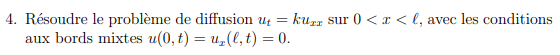
\includegraphics[scale=0.5]{img_12.png}
\end{figure}
On pose l'équation séparée

$$\frac{T'}{kT}=\frac{X''}{X}=-\lambda$$

$$T(t)=Ae^{-\lambda kt}$$
$$X(x)=A\cos(\beta x)+B\sin(\beta x)$$

$$X(0)=A + 0 = 0\longrightarrow A=0$$
$$X'(l)=B\beta\cos\left(\beta l)\right)=0\longrightarrow \begin{cases}B=0\\\beta=0\\\beta l=n\pi +\frac{\pi}{2}\end{cases}$$
On va choisir la dernière option pour éviter que le problème soit trop facile
$$\beta=\frac{n\pi +\frac{\pi}{2}}{l}=\frac{\pi\left(n+\frac{1}{2}\right)}{l}$$

$$X(x)=B\sin\left(\frac{n\pi +\frac{\pi}{2}}{l} x\right)$$

$$u(x,t)=T(t)X(x)=Ce^{-\left(\frac{n\pi +\frac{\pi}{2}}{l}\right)^2 kt}\sin\left(\frac{n\pi +\frac{\pi}{2}}{l} x\right)\qquad C=AB$$
\subsection{Série 4 - Exercice 5}
\label{S4E5}
\begin{figure}[H]
\centering
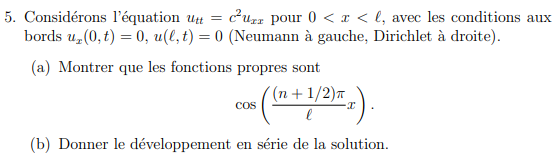
\includegraphics[scale=0.5]{img_13.png}
\end{figure}
\subsubsection{(a)}
$$\frac{X''}{X}=\frac{T''}{c^2 T}=-\lambda$$
$$\lambda=\beta^2$$
$$\begin{cases}
T(t)=A\cos(\beta ct)+B\sin(\beta ct)\\
X(x)=C\cos(\beta x)+D\sin(\beta x)
\end{cases}$$

$$X'(0)=D\beta=0\longrightarrow\begin{cases}D=0\\\beta=0\end{cases}$$
On va supposer que $D=0$, sinon le problème n'est pas intéressant

$$X(l)=C\cos(\beta l)=0\longrightarrow\begin{cases}C=0\\\beta l=n\pi+\frac{\pi}{2}\end{cases}$$
On va supposer que c'est la deuxième option, sinon le problème n'est pas intéressant

$$\beta =\frac{n\pi+\frac{\pi}{2}}{l}$$

On a donc
$$X(x)=C\cos\left(\frac{n\pi+\frac{\pi}{2}}{l} x\right)$$
\subsubsection{(b)}
$$u(x,t)=\sum_{n=0}^{\infty}\left(A\cos\left(\frac{n\pi+\frac{\pi}{2}}{l} ct\right)+B\sin\left(\frac{n\pi+\frac{\pi}{2}}{l} ct\right)\right)C\cos\left(\frac{n\pi+\frac{\pi}{2}}{l} x\right)$$
\subsection{Série 5 - Exercice 1}
\label{S5E1}
\begin{figure}[H]
\centering
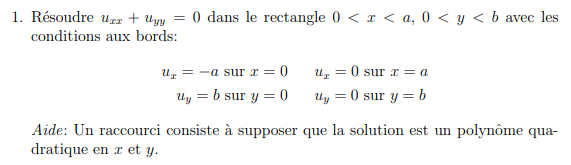
\includegraphics[scale=0.5]{img_14.png}
\end{figure}
On sais que la solution sera de la forme

$$u(x,y)=Ax^2+By^2+Cxy+Dx+Ey+F$$
On applique les conditions aux bords de manière successive. D'abord sur $x$ :
$$u_x(0,y)=-a\qquad u_x(a,y)=0$$
$$u_x(0,y)=C_y+D=-a\longrightarrow \boxed{C=0}\quad \boxed{D=-a}$$
$$u_x(a,y)=2Aa-a=0\longrightarrow \boxed{A=\frac{1}{2}}$$
Ensuite sur $y$
$$u_y(x,0)=b\qquad u_y(x,b)=0$$
$$u_y(x,0)=C_x+E=b\longrightarrow \boxed{E=b}$$
$$u_y(x,b)=2Bb+b\longrightarrow \boxed{B=-\frac{1}{2}}$$

On a directement la solution finale
$$\boxed{u(x,y)=\frac{1}{2}x^2-\frac{1}{2}y^2-ax+by+C_1\qquad C_1\in\mathbb{R}}$$
\subsection{Série 6 - Exercice 2}
\label{S6E2}
\begin{figure}[H]
\centering
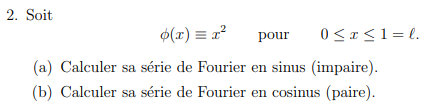
\includegraphics[scale=0.5]{img_15.png}
\end{figure}
\subsubsection{(a)}
$$\phi(x)=\sum_{n=1}^{\infty}A_n\sin\left(\frac{n\pi}{l}x\right)$$
$$A_n=\frac{2}{l}\int_{0}^{l}x^2\sin\left(\frac{n\pi x}{l}\right)dx$$
On utilise l'intégration par parties pour supprimer le $x^2$
$$A_n=\frac{2}{l}\int_{0}^{1}\underbrace{x^2}_{v}\underbrace{\sin(n\pi x)}_{u'}dx=\frac{2}{l}\left(\left(-x^2\frac{1}{n\pi}\cos(n\pi x)\right)^{1}_{0}+\int_{0}^{1}2x\frac{1}{n\pi}\cos(n\pi x)dx\right)$$
On refait une intégration par parties
$$A_n=\frac{2}{l}\left(\frac{-1}{n\pi}\cos(n\pi)+\underbrace{\left(2x\frac{1}{n^2\pi^2}\sin\left(n\pi x\right)\right)_0^1}_{0}-\int_{0}^{1}2\frac{1}{n^2\pi^2}\sin(n\pi x)dx\right)$$
on effectue l'intégrale
$$A_n=\frac{2}{l}\left(\frac{-1}{n\pi}\cos(n\pi)+\frac{2}{n^2\pi^2}\left(\frac{1}{n\pi}\cos(n\pi x)\right)_0^1\right)=\frac{-2}{n\pi}\cos(n\pi)+\frac{4}{n^3\pi^3}\left(\cos(n\pi)-1\right)$$

$$A_n=\frac{(4-2n^2\pi^2)(-1)^n-4}{n^3\pi^3}$$

On obtient donc l'équation finale

$$\boxed{\phi(x)=\sum_{n=1}^{\infty}\frac{(4-2\pi^2n^2)(-1)^n-4}{\pi^3n^3}\sin(n\pi x)}$$
\subsubsection{(b)}

Comme avant on pose les équations de base

$$\phi(x)=\frac{A_0}{2}+\sum_{n=1}^{\infty}A_n\cos(n\pi x)$$
$$A_n=2\int_{0}^{1}\phi(x)\cos(n\pi x)dx$$
On commence par déterminer $A_0$ qui est facile
$$A_0=2\int_{0}^{1}x^2dx=2\left(\frac{x^3}{3}\right)^{1}_{0}=\frac{2}{3}$$
On fait une intégration par parties
$$A_n=2\int_{0}^{1}\underbrace{x^2}_{v}\underbrace{\cos(n\pi x)}_{u'}dx=2\left(\underbrace{\left(x^2\frac{1}{n\pi}\sin(n\pi x)\right)^{1}_{0}}_{0}-\int_{0}^{1}2x\frac{1}{n\pi}\sin(n\pi x)dx\right)$$
On peut simplifier puis on refait une intégration par parties
$$A_n=\frac{-4}{n\pi}\int_{0}^{1}\underbrace{x}_{v}\underbrace{\sin(n\pi x)}_{u'}dx=\frac{-4}{n\pi}\left(\left(-x\frac{1}{n\pi}\cos(n\pi x)\right)_{0}^{1}+\int_{0}^{1}\frac{1}{n\pi}\cos(n\pi x)dx\right)$$

$$A_n=\frac{-4}{n^2\pi^2}\left(\underbrace{(-x\cos(n\pi x))^{1}_{0}}_{-\cos(n\pi}+\underbrace{\left(\frac{1}{n\pi}\sin(n\pi x)\right)_{0}^{1}}_{0}\right)$$

On a donc finalement

$$A_n=\frac{4(-1)^n}{n^2\pi^2}$$

Et l'équation finale

$$\boxed{\phi(x)=\frac{1}{3}+\sum_{n=1}^{\infty}\frac{4(-1)^n}{n^2\pi^2}\cos(n\pi x)}$$
\subsection{Série 6 - Exercice 5}
\label{S6E5}
\begin{figure}[H]
\centering
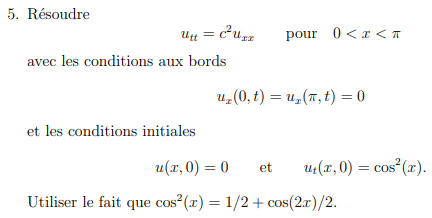
\includegraphics[scale=0.5]{img_16.png}
\end{figure}
On utilise la solution générale de l'équation d'onde pour un problème avec conditions aux bords de Neumann ($u_x(0,t)=u_x(l,t)=0$)

$$u(x,t)=\frac{1}{2}A_0+\frac{1}{2}B_0t+\sum_{n=1}^{\infty}\left(A_n\cos\left(\frac{n\pi c}{l}t\right)+B_n\sin\left(\frac{n\pi c}{l}t\right)\right)\cos\left(\frac{n\pi}{l}x\right)$$
Avec les conditions initiales
$$\phi(x)=u(x,0)=\frac{1}{2}A_0+\sum_{n=1}^{\infty}A_n\cos\left(\frac{n\pi}{l}x\right)$$
$$\psi(x)=u_t(x,0)=\frac{1}{2}B_0+\sum_{n=1}^{\infty}\frac{n\pi c}{l}B_n\cos\left(\frac{n\pi}{l}x\right)$$

On applique les conditions initiales
$$u(x,0)=\frac{1}{2}A_0+\sum_{n=1}^{\infty}A_n\cos\left(\frac{n\pi}{l}x\right)=0\longrightarrow \boxed{\begin{cases}A_0=0\\A_n=0\end{cases}}$$

$$u_t(x,0)=\frac{1}{2}B_0+\sum_{n=1}^{\infty}\frac{n\pi c}{l}B_n\cos\left(\frac{n\pi}{l}x\right)=\frac{1}{2}+\frac{\cos(2x)}{2}$$
$$\frac{1}{2}B_0=\frac{1}{2}\longrightarrow\boxed{B_0=1}$$

$$\sum_{n=1}^{\infty}\frac{n\pi c}{l}B_n\cos\left(\frac{n\pi}{l}x\right)=\frac{\cos(2x)}{2}$$
On a $n=2$ et $l=\pi$
$$\frac{2\pi c}{\pi}B_2\cos\left(\frac{2\pi}{\pi}x\right)=\frac{\cos(2x)}{2}$$

$$2cB_2\cos\left(2x\right)=\frac{\cos(2x)}{2}$$

$$2cB_2=\frac{1}{2}$$
$$4cB_2=1$$
$$\boxed{B_2=\frac{1}{4c}}$$

On écrit donc la solution finale

$$\boxed{u(x,t)=\frac{1}{2}t+\frac{1}{4c}\sin(2ct)\cos(2x)}$$
\subsection{Série 7 - Exercice 4}
\label{S7E4}
\begin{figure}[H]
\centering
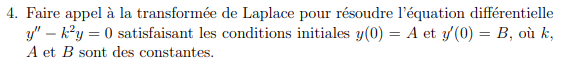
\includegraphics[scale=0.5]{img_17.png}
\end{figure}
$$s^2Y(s)-sy(0)-y'(0)-k^2Y(s)=0$$
$$Y(s)(s^2-k^2)=sy(0)+y'(0)$$
$$Y(s)=\frac{sy(0)}{s^2-k^2}+\frac{y'(0)}{s^2-k^2}=A\frac{s}{s^2-k^2}+\frac{B}{k}\frac{k}{s^2-k^2}$$

$$\boxed{y(t)=A\cosh(kt)+\frac{B}{k}\sinh(kt)}$$


\end{multicols}
\end{document}